\chapter{The Integrated Discovery Pipeline}
\label{sec:discovery_pipeline}

The complete computational pipeline integrates generation, validation, filtering, and prediction into an end-to-end workflow for polymer discovery. Given a target pharmaceutical molecule (e.g., aspirin, ibuprofen, or metformin), the pipeline proceeds as follows.

First, the target molecule is converted to SMILES notation using the PubChem database. Second, the generative model produces a batch of candidate polymer P-SMILES strings. Third, invalid and duplicate structures are eliminated through validation. Fourth, the heuristic filters based on logP, TPSA, FMO gaps, and SA score are applied. Fifth, the MLP predicts the adsorption capacity for each surviving candidate. Finally, candidates are ranked by predicted capacity, and those exceeding a specified threshold are returned as promising discoveries.

This pipeline was tested with multiple target molecules, demonstrating its ability to identify candidate polymers with predicted capacities in excess of 1.0 mg/g. Visualization of capacity versus concentration and pH provides additional insight into how the predicted performance varies with experimental conditions, guiding the design of laboratory validation experiments.
\begin{figure}[htbp]
	\centering
	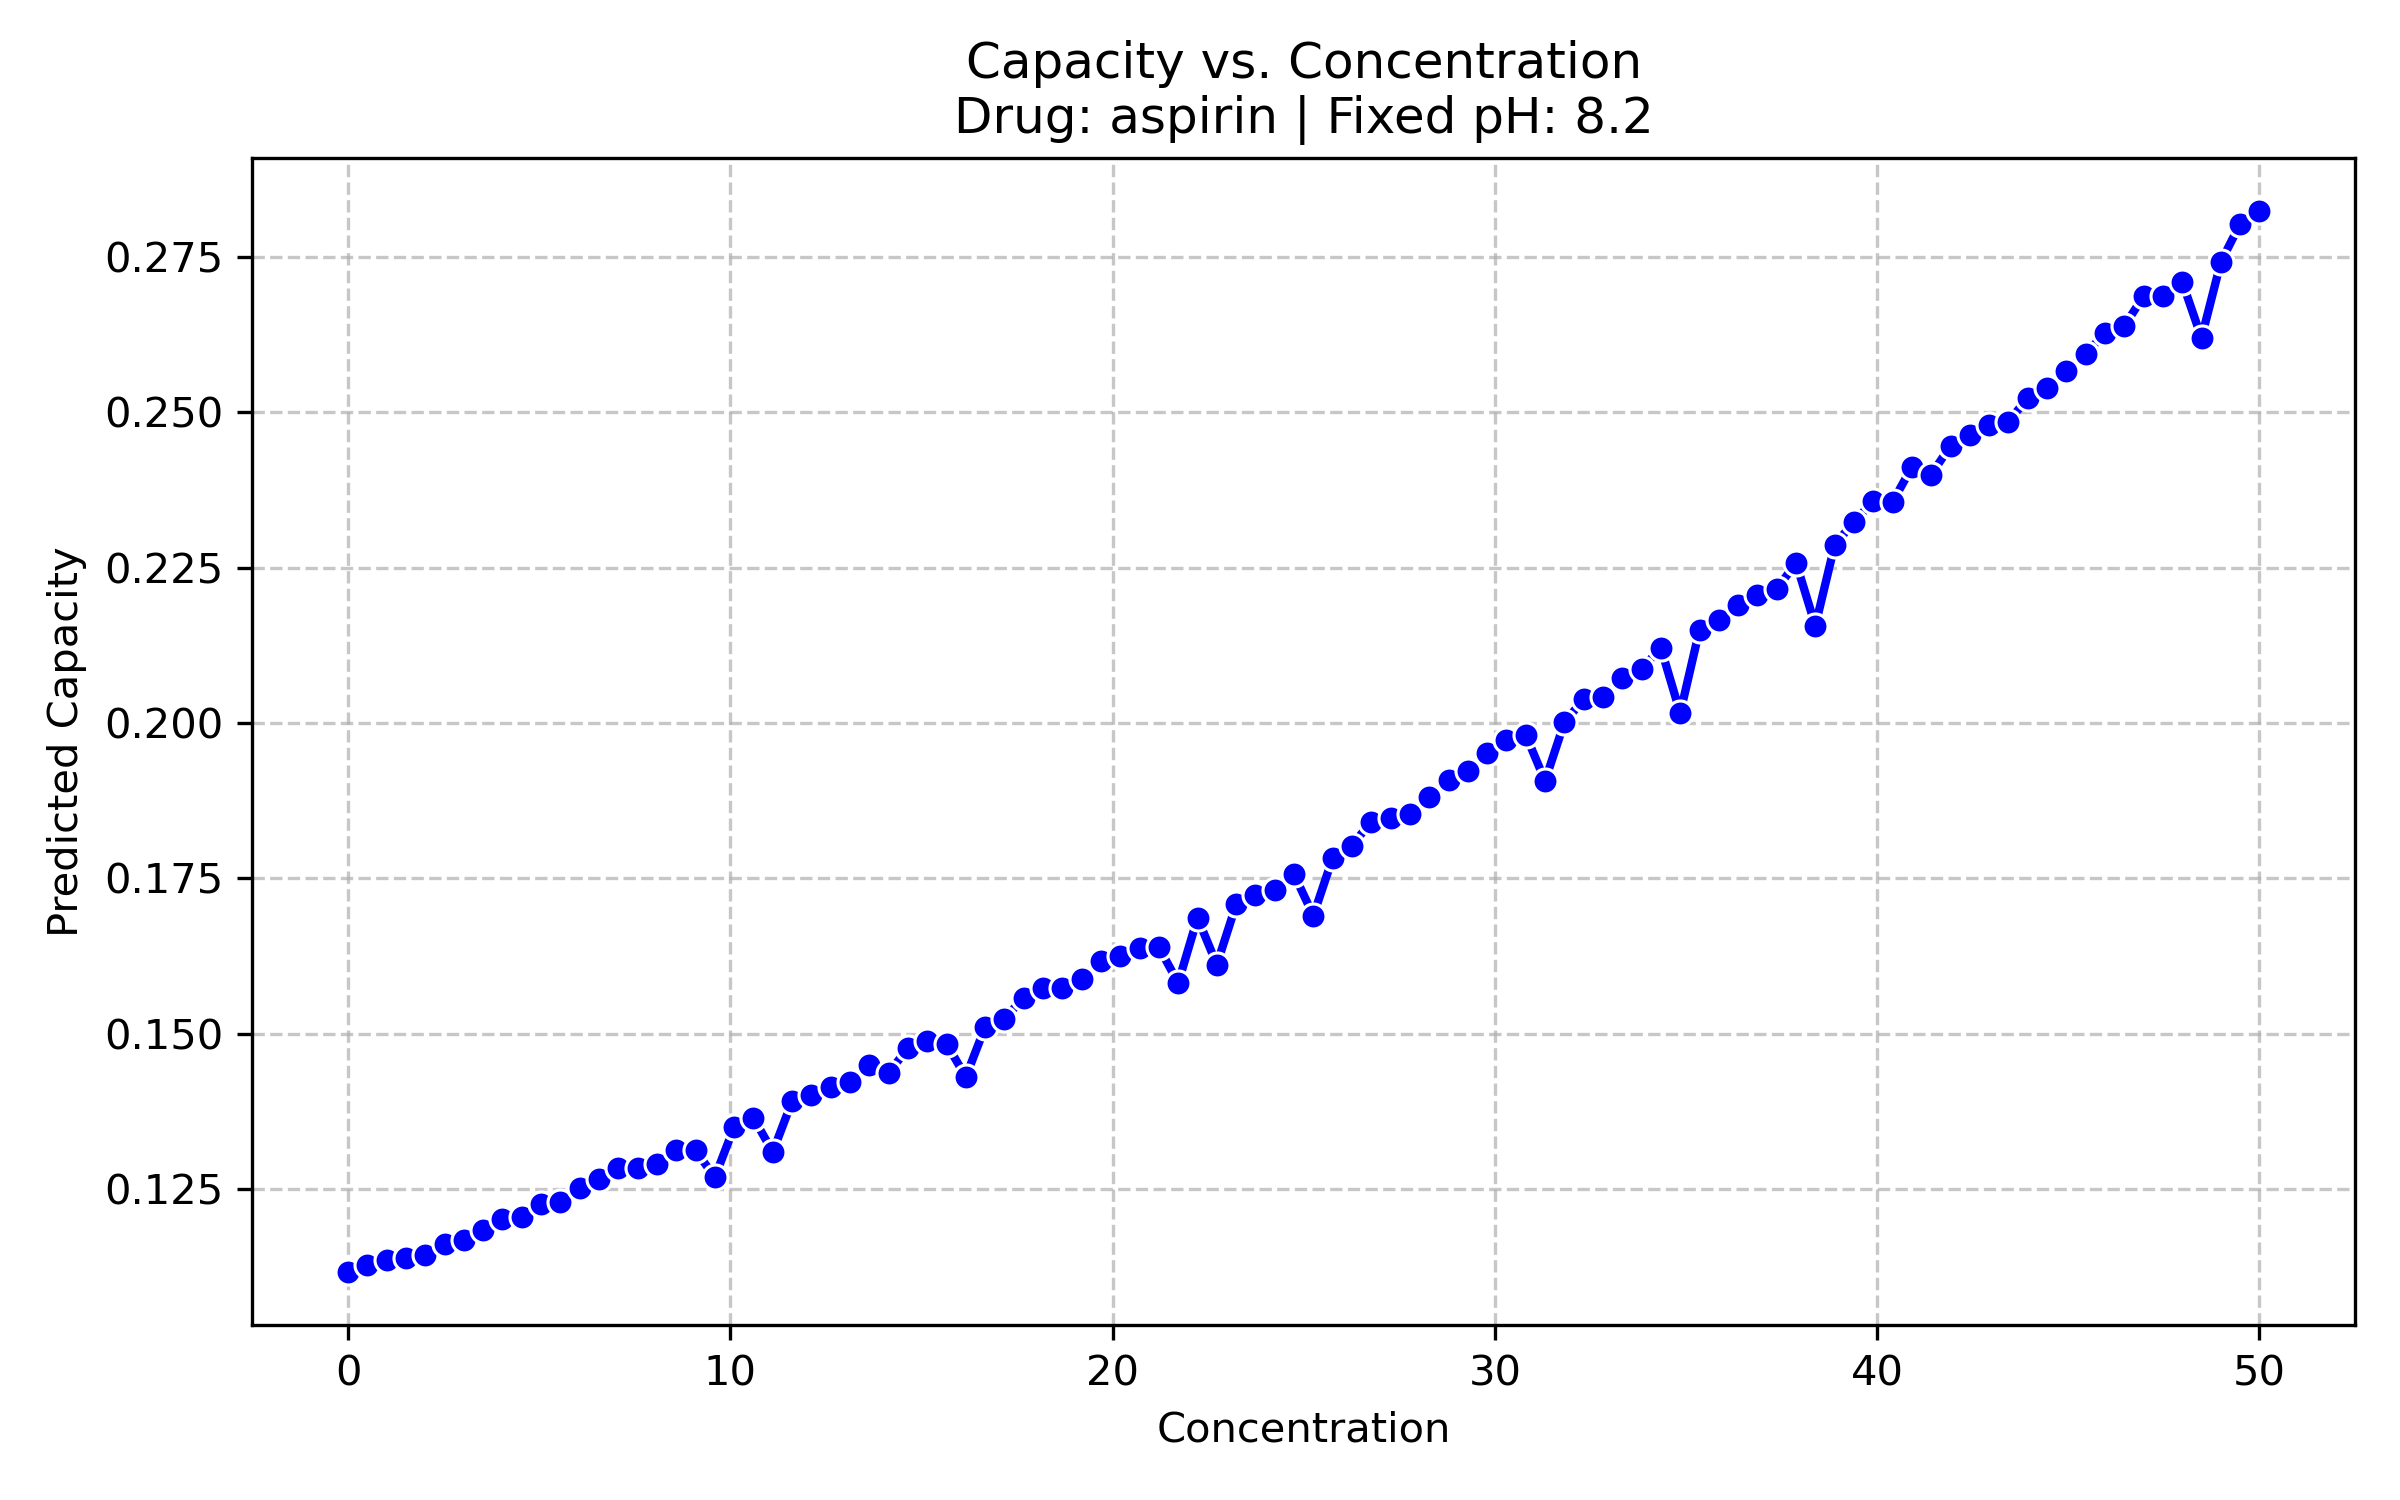
\includegraphics[width=0.75\textwidth]{RESULTS/predicted_capacities/plot_conc_aspirin.png}
	\caption{Predicted adsorption capacity vs. initial concentration for the top-ranked polymer against aspirin.}
	\label{fig:pipeline_conc_aspirin}
\end{figure}
\begin{figure}[htbp]
	\centering
	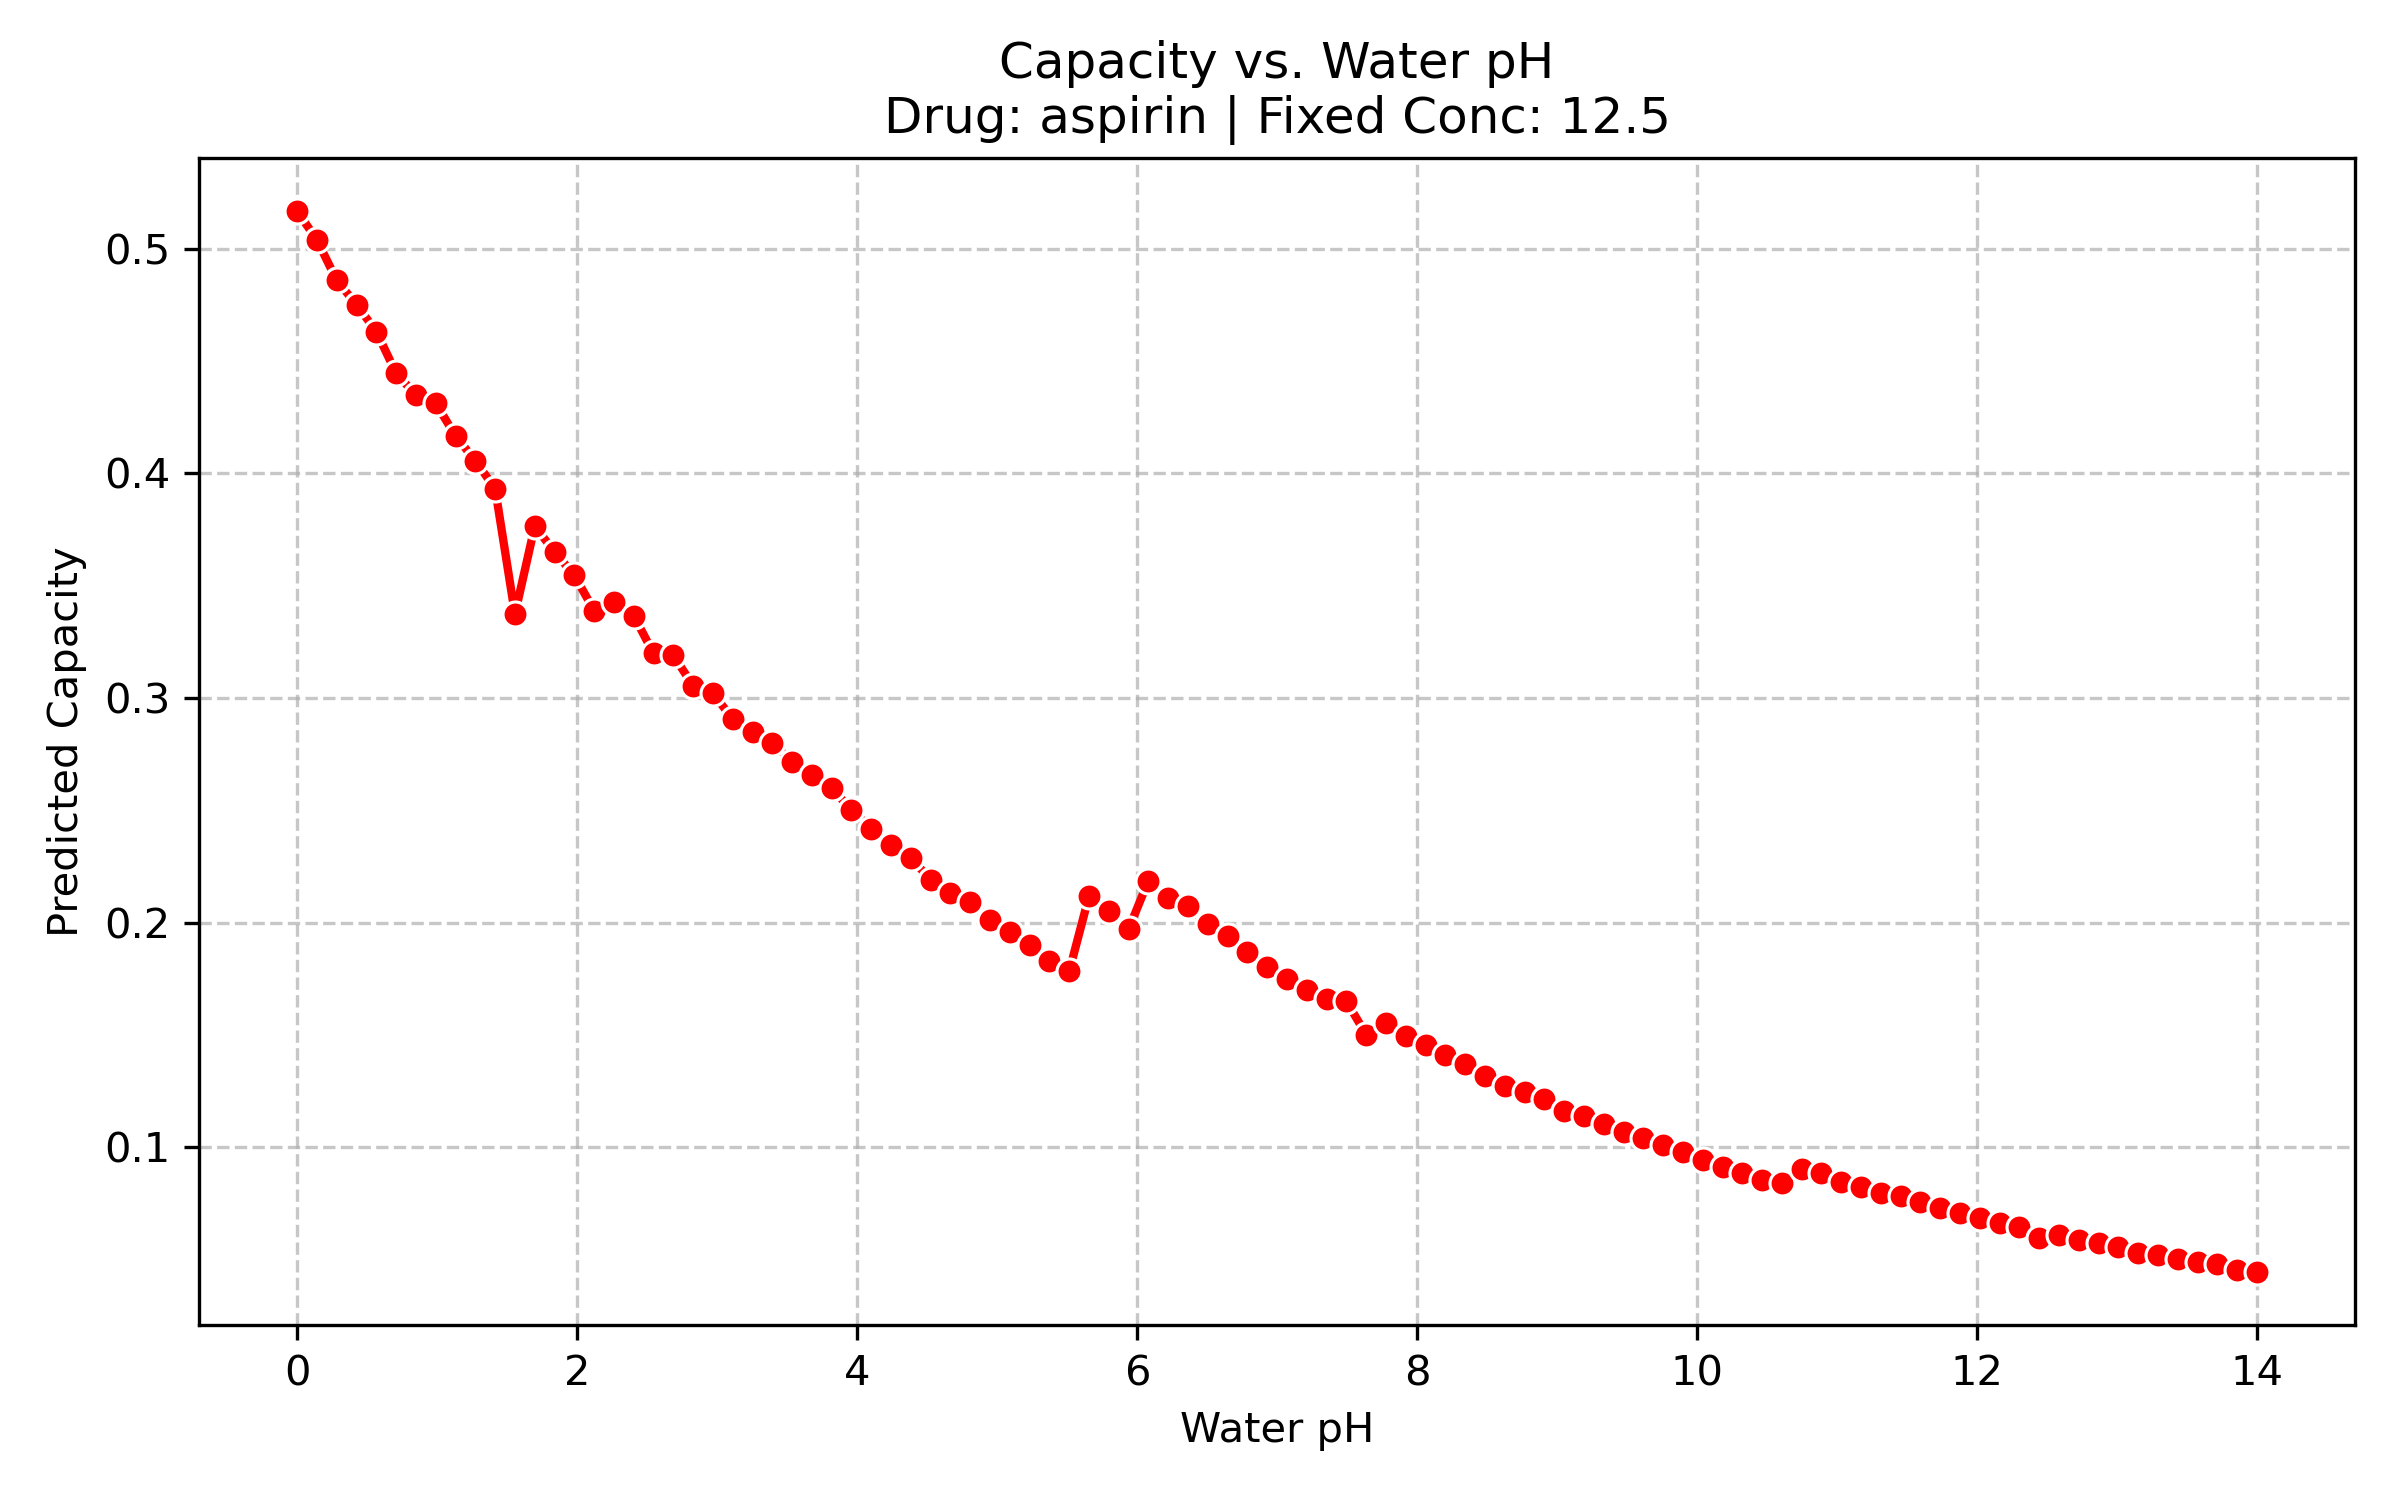
\includegraphics[width=0.75\textwidth]{RESULTS/predicted_capacities/plot_ph_aspirin.png}
	\caption{Predicted adsorption capacity vs. water pH for the top-ranked polymer against aspirin.}
	\label{fig:pipeline_ph_aspirin}
\end{figure}
The pipeline is configurable, allowing adjustment of generation parameters (temperature, batch size), filter thresholds, and the target capacity cutoff. This flexibility enables adaptation to different application contexts, such as targeting different pollutant classes or optimizing for specific environmental conditions.
